
    \begin{figure}[hp]
    \centering
<<<<<<< HEAD
	\captionsetup{justification=justified, singlelinecheck=false, width=1\textwidth}
    \caption{Mapa da região de interesse no entorno do empreendimento, mostrando as principais cidades, rodovias e rios, com a localização das pedreiras, estação \textbf{SP7}, e eventos próximos ao empreendimento detectados no período de interesse.}
=======
    \captionsetup{justification=justified, singlelinecheck=false, width=1\textwidth}
    \caption{Mapa da região de interesse no entorno do empreendimento, mostrando as principais cidades, rodovias e rios, com a localização das pedreiras, estações \textbf{BCM2} e \textbf{MC9}, e eventos próximos ao empreendimento detectados no período de interesse.}
>>>>>>> 157db0ea11ef4bcaca122b47262699549e3e7111
    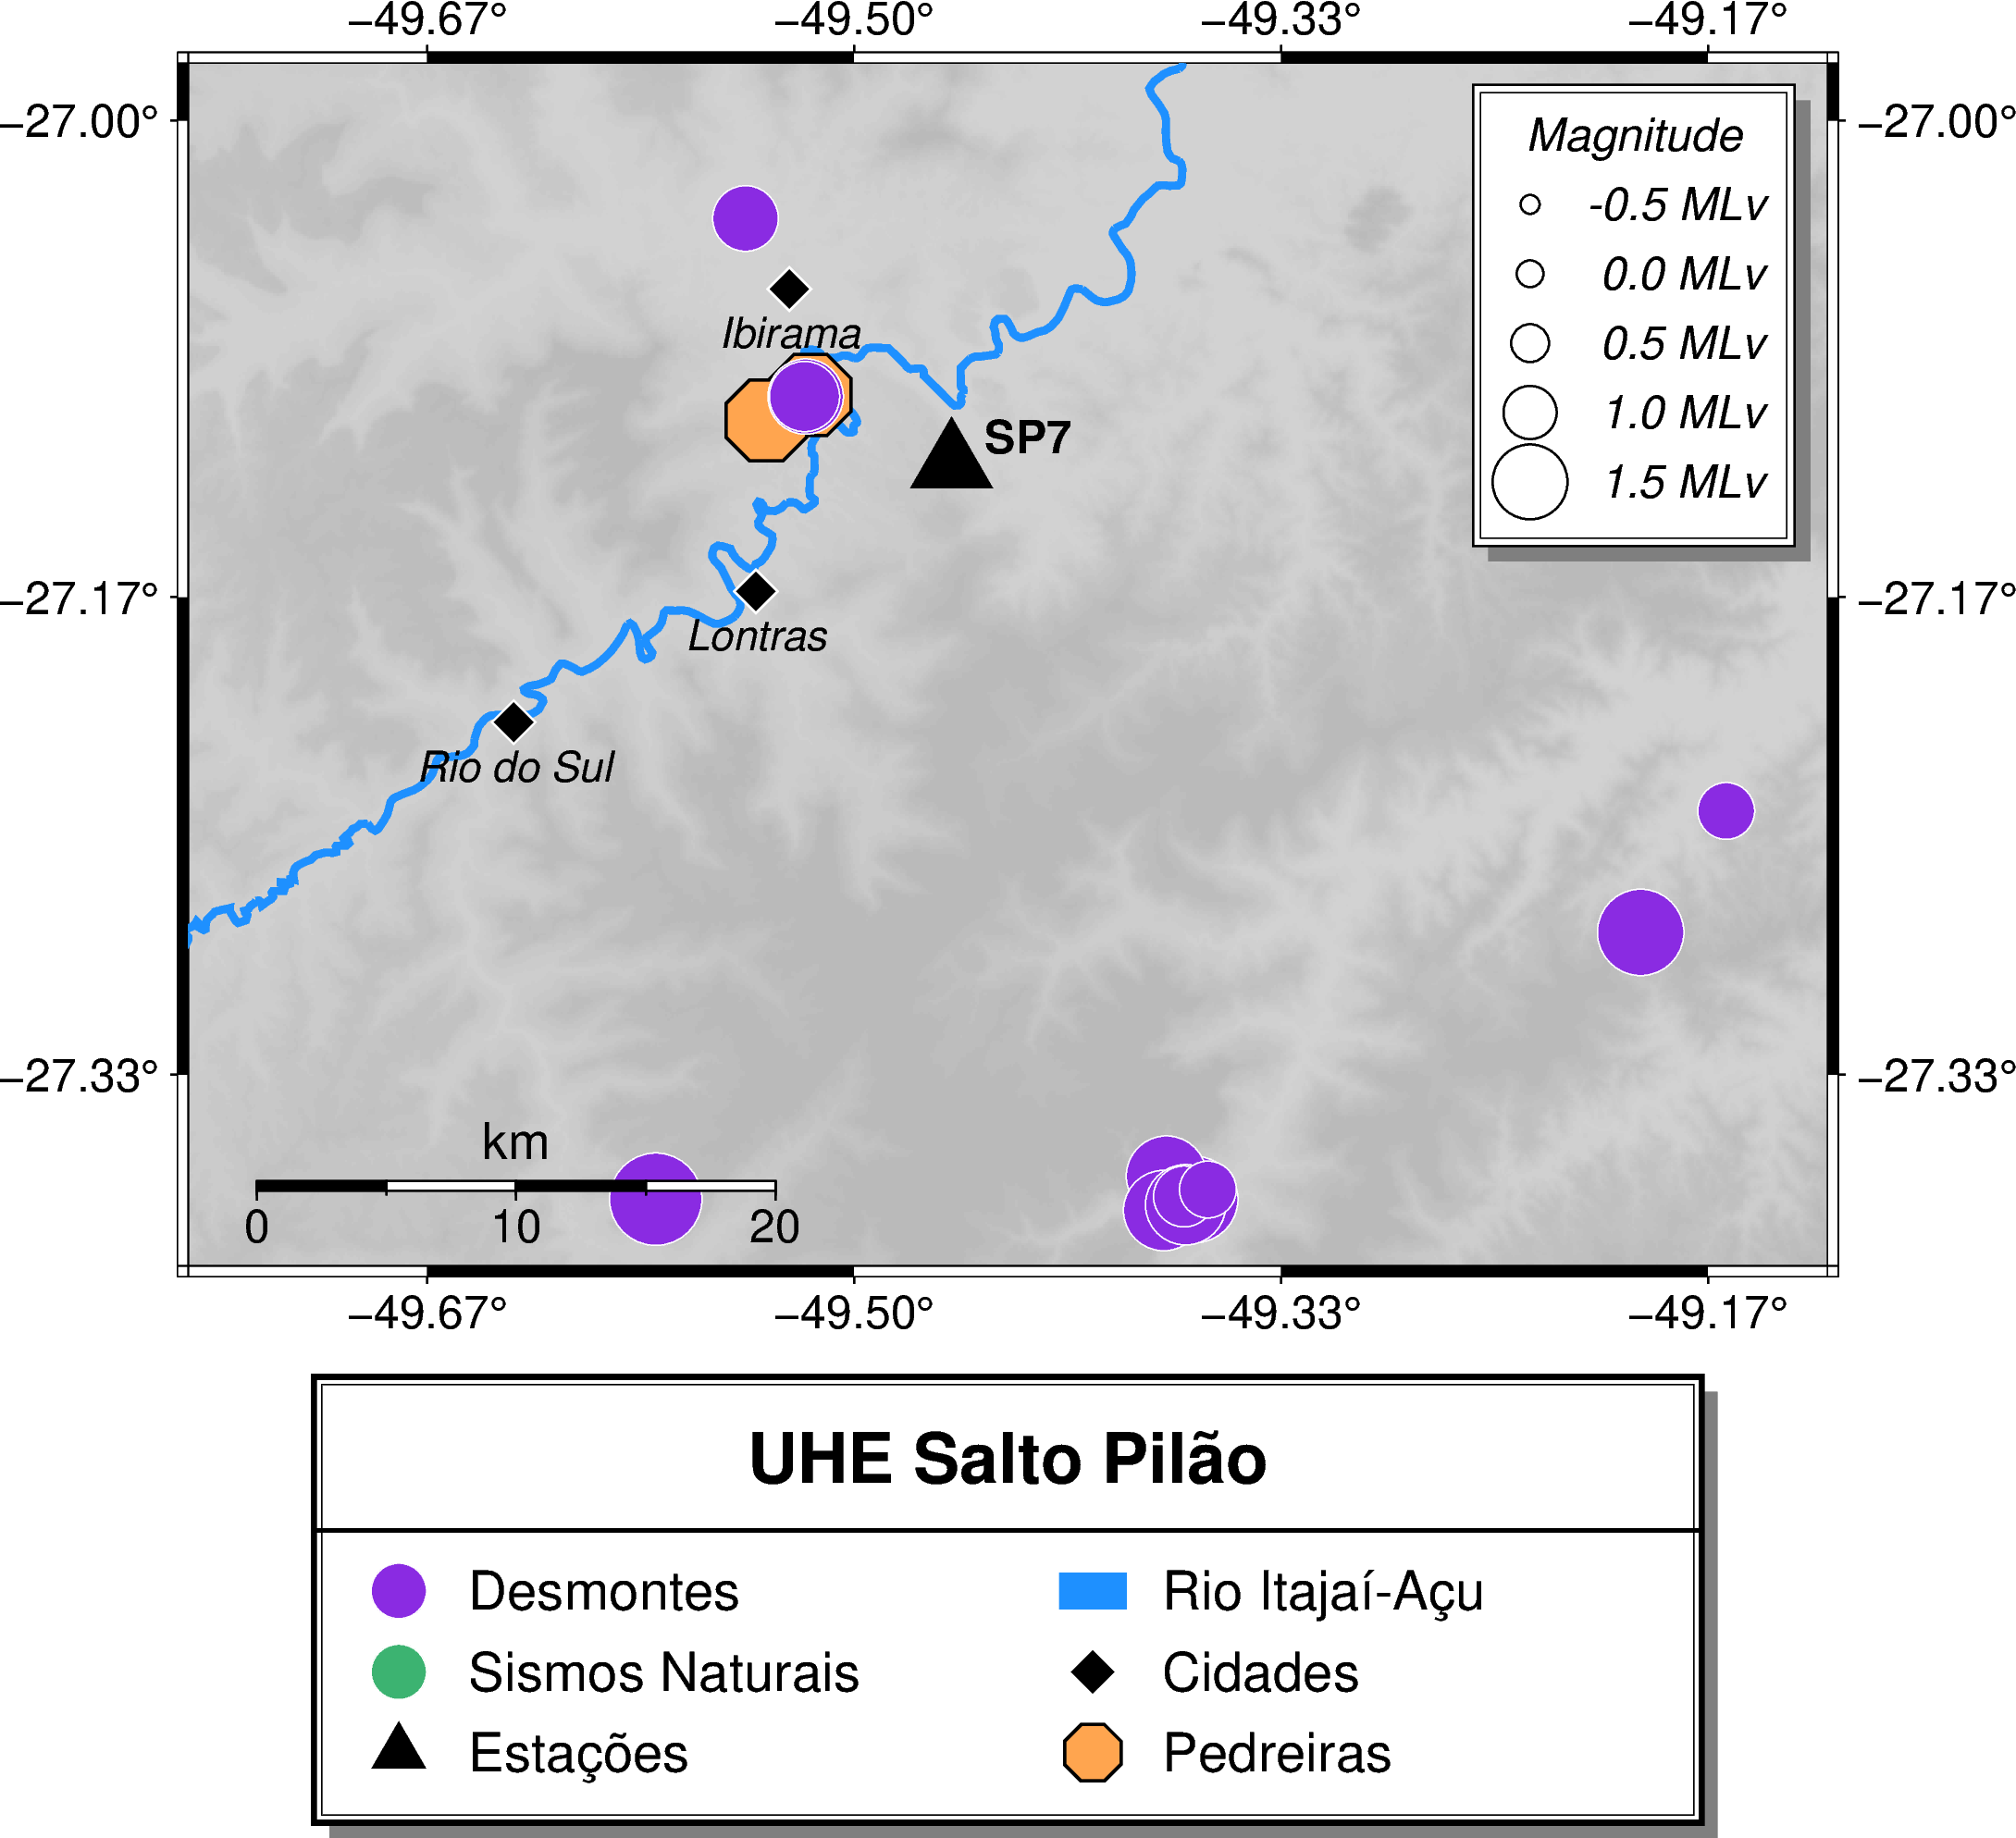
\includegraphics[width=1.0\textwidth]{./boletim/main/figuras/mapaevents.png}
    \caption*{Fonte: IPT}
    \end{figure}
    \newpage
    